\subsubsection{Dinic (Fluxo Máximo Eficiente)}
O algoritmo de Dinic utiliza o conceito de \textit{grafo de níveis} (construído
via BFS) para encontrar caminhos de aumento e \textit{fluxos bloqueantes}
(encontrados via DFS) em camadas. Sua complexidade de tempo é $\mathcal{O}(V^2
    E)$, sendo extremamente rápido em grafos gerais.

\paragraph{Pseudo-Código: }\mbox{}\\
\begin{algorithm}[H]
    \SetAlgoLined
    \SetKwFunction{Dinic}{Dinic}
    \SetKwProg{Fn}{Função}{:}{}

    \Fn{\Dinic{$s, t, adj$}}{
        $fluxoMaximo \gets 0$\;
        \While{\text{BFS constrói o grafo de níveis a partir de } $s$ \text{ até } $t$}{
            \While{\text{encontrar caminho de fluxo bloqueante com DFS}}{
                $fluxoMaximo \gets fluxoMaximo + \text{fluxoEncontrado}$\;
            }
        }
        \Retorna $fluxoMaximo$\;
    }
    \caption{Algoritmo de Dinic}
\end{algorithm}

Veja o Dinic construindo o grafo de níveis e encontrando o fluxo bloqueante:\\
\vspace{0.5cm} \noindent
\begin{minipage}[t]{0.31\textwidth}
    \centering
    \textbf{Passo 1: Rede Residual}\\
    \vspace{0.2cm}
    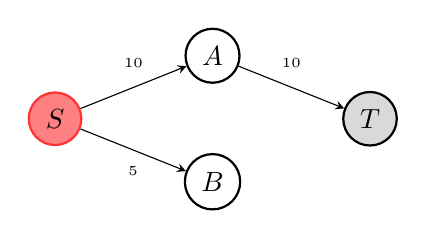
\begin{tikzpicture}[every node/.style={circle, draw, minimum size=0.5cm, thick}, >=stealth]
        \node[fill=red!50, draw=red!80] (S) at (-1, 0) {$S$};
        \node (A) at (1, 0.8) {$A$};
        \node (B) at (1, -0.8) {$B$};
        \node[fill=gray!30] (T) at (3, 0) {$T$};
        \draw[->] (S) -- node[above, draw=none, fill=none] {\tiny 10} (A);
        \draw[->] (S) -- node[below, draw=none, fill=none] {\tiny 5} (B);
        \draw[->] (A) -- node[above, draw=none, fill=none] {\tiny 10} (T);
    \end{tikzpicture}

    \vspace{0.2cm}
    \footnotesize
    \raggedright
    Rede inicial com capacidades nas arestas entre a fonte $S$ e o sumidouro $T$.
\end{minipage}%
\hfill
%
\begin{minipage}[t]{0.31\textwidth}
    \centering
    \textbf{Passo 2: Grafo de Níveis (BFS)}\\
    \vspace{0.2cm}
    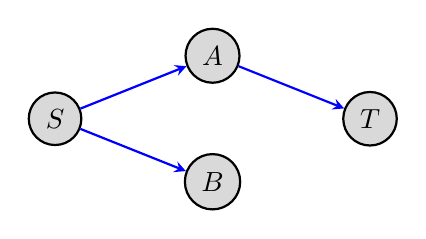
\begin{tikzpicture}[every node/.style={circle, draw, minimum size=0.5cm, thick}, >=stealth]
        \node[fill=gray!30] (S) at (-1, 0) {$S$};
        \node[fill=gray!30] (A) at (1, 0.8) {$A$};
        \node[fill=gray!30] (B) at (1, -0.8) {$B$};
        \node[fill=gray!30] (T) at (3, 0) {$T$};
        \draw[->, blue, thick] (S) -- (A);
        \draw[->, blue, thick] (S) -- (B);
        \draw[->, blue, thick] (A) -- (T);
    \end{tikzpicture}

    \vspace{0.2cm}
    \footnotesize
    \raggedright
    BFS atribui níveis aos nós ($level[S]=0, level[A]=1, level[T]=2$).
\end{minipage}%
\hfill
%
\begin{minipage}[t]{0.31\textwidth}
    \centering
    \textbf{Passo 3: Fluxo Bloqueante (DFS)}\\
    \vspace{0.2cm}
    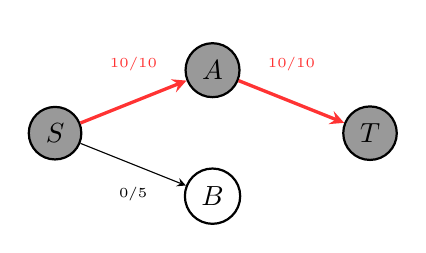
\begin{tikzpicture}[every node/.style={circle, draw, minimum size=0.5cm, thick}, >=stealth]
        \node[fill=gray!80] (S) at (-1, 0) {$S$};
        \node[fill=gray!80] (A) at (1, 0.8) {$A$};
        \node (B) at (1, -0.8) {$B$};
        \node[fill=gray!80] (T) at (3, 0) {$T$};
        \draw[->, red!80, very thick] (S) -- node[above, draw=none, fill=none] {\tiny 10/10} (A);
        \draw[->] (S) -- node[below, draw=none, fill=none] {\tiny 0/5} (B);
        \draw[->, red!80, very thick] (A) -- node[above, draw=none, fill=none] {\tiny 10/10} (T);
    \end{tikzpicture}

    \vspace{0.2cm}
    \footnotesize
    \raggedright
    DFS envia fluxo pelas camadas até que nenhuma rota adicional seja possível.
\end{minipage}

\vspace{0.3cm}

\paragraph{Implementação: }\mbox{}\\
\textbf{C++ (Estrutura Completa de Dinic):}
\begin{lstlisting}[language=C++]
struct Edge {
    int to;
    long long cap;
    long long flow;
    int rev;
};

struct Dinic {
    int n;
    vector<vector<Edge>> adj;
    vector<int> level, ptr;

    Dinic(int n) : n(n), adj(n), level(n), ptr(n) {}

    void add_edge(int from, int to, long long cap) {
        adj[from].push_back({to, cap, 0, (int)adj[to].size()});
        adj[to].push_back({from, 0, 0, (int)adj[from].size() - 1});
    }

    bool bfs(int s, int t) {
        fill(level.begin(), level.end(), -1);
        level[s] = 0;
        queue<int> q;
        q.push(s);
        while (!q.empty()) {
            int v = q.front();
            q.pop();
            for (auto& edge : adj[v]) {
                if (edge.cap - edge.flow > 0 && level[edge.to] == -1) {
                    level[edge.to] = level[v] + 1;
                    q.push(edge.to);
                }
            }
        }
        return level[t] != -1;
    }

    long long dfs(int v, int t, long long pushed) {
        if (pushed == 0) return 0;
        if (v == t) return pushed;
        for (int& cid = ptr[v]; cid < adj[v].size(); ++cid) {
            auto& edge = adj[v][cid];
            int tr = edge.to;
            if (level[v] + 1 != level[tr] || edge.cap - edge.flow == 0) continue;
            long long tr_pushed = dfs(tr, t, min(pushed, edge.cap - edge.flow));
            if (tr_pushed == 0) continue;
            edge.flow += tr_pushed;
            adj[tr][edge.rev].flow -= tr_pushed;
            return tr_pushed;
        }
        return 0;
    }

    long long max_flow(int s, int t) {
        long long flow = 0;
        while (bfs(s, t)) {
            fill(ptr.begin(), ptr.end(), 0);
            while (long long pushed = dfs(s, t, 1e18)) {
                flow += pushed;
            }
        }
        return flow;
    }
};
\end{lstlisting}
\newpage